\chapter{Theoretische Grundlagen}
\label{background}

%- Allgemeine Wissensgrundlagen des Fachgebiets
%- Spezielle Grundlagen, die für das Verständnis erforderlich sind
%- Rahmenbedingungen für die Arbeit
%- Ausführungen zum Stand des Wissens / der Technik
%Als Leitprinzip gilt: Nur Informationen erwähnen, die
%- später benötigt werden,
%- notwendig sind, um die Arbeit oder ihre Motivation zu verstehen
%Das heißt insbesondere,
%- keine Inhalte aus Lehrbüchern, außer
%- diese werden benötigt, um Problemstellung oder Lösungsweg zu definieren.

Ziel des nachfolgenden Kapitels soll es sein, eine allgemeine Wissensgrundlage über wesentliche Begrifflichkeiten im Thema zu schaffen. Um die nachfolgenden Ausführungen im Hauptteil (vgl. \ref{problemfields} und \ref{agilepractices}) besser nachvollziehen zu können, sollen wichtige Definitionen und Begriffsabgrenzungen vorgenommen werden.

\section{Digitale Transformation}

\begin{figure}[H]
	\centering
	\fbox{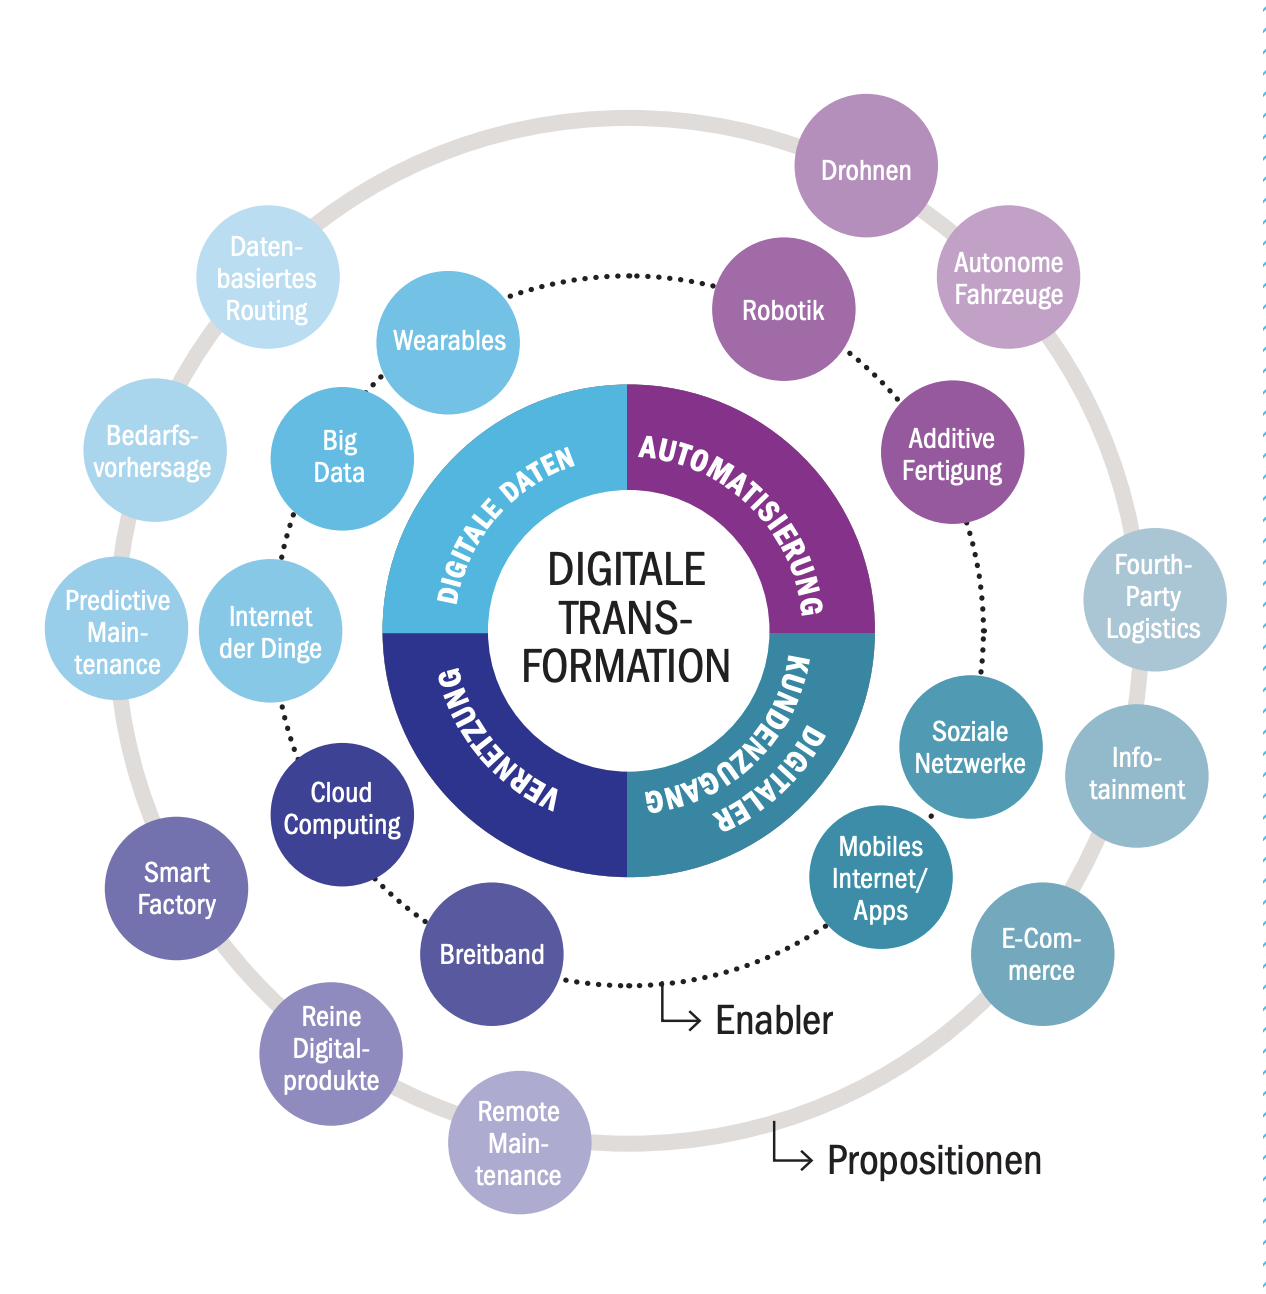
\includegraphics[width=0.7\linewidth]{pics/dtbigpicture}}
	\caption[Big-Picture der Digitalen Transformation]{Treiber der Digitalen Transformation \protect \cite[S. 20]{bloching_digitale_2015}}
	\label{fig:bigpicture}
\end{figure}

\todots

\section{Change Management}

\todots

\section{Agilität}

\todots

\section{Agile Organisation}

\todots

\section{Agile Transformation}

\todots

\section{Abgrenzung Großunternehmen}